\documentclass[10pt]{article}
\usepackage[utf8]{inputenc}
\usepackage[T1]{fontenc}
\usepackage{amsmath}
\usepackage{amsfonts}
\usepackage{amssymb}
\usepackage[version=4]{mhchem}
\usepackage{stmaryrd}
\usepackage{graphicx}
\usepackage[export]{adjustbox}
\graphicspath{ {./images/} }

\begin{document}

    In a binary system involving a compact star, where the companion star does not overflow its Roche lobe, the primary source of accretion for the compact star is the stellar wind from the companion star. This wind-fed accretion is especially significant in systems that include an early-type star (such as an O or B star, indicated henceforth as an OB star), alongside a compact object like a neutron star (NS) in a close orbit.

    Consider such a NS-OB star binary system where a neutron star of mass $M_{\mathrm{NS}}=2.0 \mathrm{M}_{\odot}$ and radius $R_{\mathrm{NS}}=11 \mathrm{~km}$ is orbiting in a circular orbit of radius $a$ around the centre of the OB star with velocity $v_{\text {orb }}=1.5 \times 10^{5} \mathrm{~m} \mathrm{~s}^{-1}$ (see figure below). Throughout this problem the mass loss from the OB star is assumed to be spherically symmetric and its rate is $\dot{M}_{\mathrm{OB}}=1.0 \times 10^{-4} \mathrm{M}_{\odot} \mathrm{yr}^{-1}$.\\
    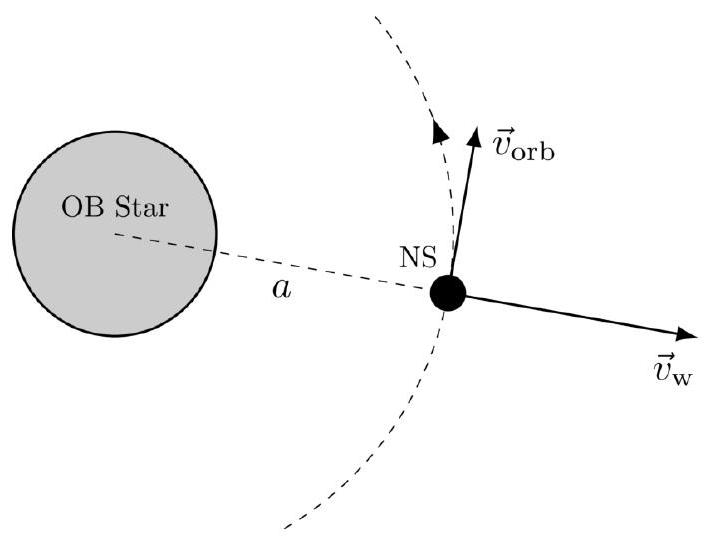
\includegraphics[max width=\textwidth, center]{2025_08_23_e94579452776a99c4850g-06}\\
    (T07.1) The accretion radius, $R_{\text {acc }}$, is defined as the maximum distance from the NS at which the stellar wind can be captured by the NS. If the stellar wind speed at the orbital distance of the NS is $v_{\mathrm{w}}= 3.0 \times 10^{6} \mathrm{~m} \mathrm{~s}^{-1}$, find $R_{\text {acc }}$ for the above system in km using standard escape velocity calculation.\\
    (T07.2) Assuming that all captured material is accreted by the NS, estimate the mass accretion rate, $\dot{M}_{\text {acc }}$, from the stellar wind onto the NS in units of $\mathrm{M}_{\odot} \mathrm{yr}^{-1}$ if $a=0.5 \mathrm{au}$. Neglect the effects of radiation pressure and finite cooling time of the accreting gas.\\
    (T07.3) Now consider the situation where the stellar wind speed at the orbital distance $a$ (near the NS) becomes comparable with orbital speed of the NS. The mass accretion rate from the stellar wind onto the NS in this case would be given by an expression of the form $\dot{M}_{\text {acc }}=\dot{M}_{\text {OB }} f(\tan \beta, q)$, where $q=M_{\mathrm{NS}} / M_{\mathrm{OB}}$ is the mass ratio of the binary and $\beta$ is the angle in the frame of the NS between the wind velocity direction and radial direction away from the OB star. Obtain the expression for $f(\tan \beta, q)$ assuming $M_{\mathrm{OB}} \gg M_{\mathrm{NS}}$.\\
    (T07.4) Consider that the fully ionized material accretes radially and is hindered due to the strong magnetic field $\vec{B}$ of the NS. This effect can be modelled as a pressure, given by $\frac{B^{2}}{2 \mu_{0}}$. We shall assume that the NS has a dipole magnetic field whose magnitude in the equatorial plane varies with the distance $r$ from the NS for $r \gg R_{\mathrm{NS}}$ as
    
    $$
    B(r)=B_{0}\left(\frac{R_{\mathrm{NS}}}{r}\right)^{3}
    $$
    
    where $B_{0}$ is the magnetic field at the equator of the NS. Assume that the axis of the magnetic dipole aligns with the rotation axis of the NS.\\
    (T07.4a) Obtain the magnetic pressure, $P_{\text {eq, mag }}$, in the equatorial plane in terms of $B_{0}, R_{\mathrm{NS}}, r, \quad[1]$ and other suitable constants.\\
    (T07.4b) The maximum distance where the accretion flow is stopped by the magnetic field at the equatorial plane is called the magnetospheric radius $R_{\mathrm{m}}$. This flow of matter will exert a pressure due to the relative motion between incoming stellar wind and the NS. Obtain an approximate expression for the critical magnetic field $B_{0, \mathrm{c}}$ for which $R_{\mathrm{m}}$ coincides with $R_{\text {acc }}$ and calculate its value in Tesla. Magnetic effects are neglected for $r>R_{\mathrm{m}}$ and consider $v_{\mathrm{w}} \gg v_{\text {orb }}$.

\end{document}